\documentclass[11pt]{article}
\usepackage[usenames]{color} %used for font color
\usepackage{amssymb} %maths
\usepackage{amsmath} %maths

\usepackage[no-math]{fontspec}
\usepackage{unicode-math}
\usepackage{libertinus}

\usepackage{pgf,xcolor}
\definecolor{itwm_blue_04}{HTML}{005A94}
\definecolor{itwm_red}{HTML}{C00000}

\usepackage{tikz}
\usetikzlibrary{shapes.misc, shadows, decorations, arrows}
\usetikzlibrary{backgrounds}
\usetikzlibrary{calc}
\usepackage{pgfplots}
\pgfplotsset{compat=newest}
\usepgfplotslibrary{fillbetween}
\usepackage{tikzpagenodes}
\usetikzlibrary{decorations.markings}\begin{document}
\begin{align*}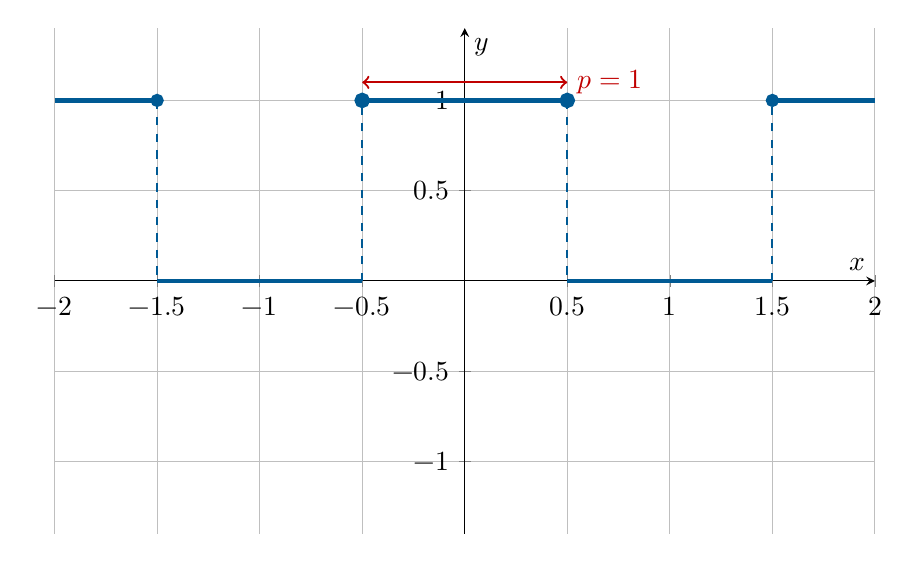
\begin{tikzpicture}
\begin{axis}[
    domain=-2:2,
    axis lines = center,
    xlabel = {$x$},
    ylabel = {$y$},
    height=8cm, width=12cm, 
    xmin=-2, xmax=2, ymin=-1.4, ymax=1.4, 
    xtick={-2, -1.5,...,2},
    ytick={-1,-0.5,...,1},
    grid = both
]
\path [name path=xaxis]
      (\pgfkeysvalueof{/pgfplots/xmin},0) --
      (\pgfkeysvalueof{/pgfplots/xmax},0);
\addplot [color=itwm_blue_04, ultra thick] coordinates {(-2,1) (-1.5, 1)};
\addplot [color=itwm_blue_04, thick, dashed] coordinates {(-1.5,1) (-1.5, 0)};
\addplot [color=itwm_blue_04, ultra thick] coordinates {(-1.5,0) (-0.5, 0)};
\addplot [color=itwm_blue_04, thick, dashed] coordinates {(-0.5,0) (-0.5, 1)};
\addplot [color=itwm_blue_04, ultra thick, mark=*] coordinates {(-0.5,1) (0.5, 1)};
\addplot [color=itwm_blue_04, thick, dashed] coordinates {(0.5,1) (0.5, 0)};
\addplot [color=itwm_blue_04, ultra thick] coordinates {(0.5,0) (1.5, 0)};
\addplot [color=itwm_blue_04, thick, dashed] coordinates {(1.5,0) (1.5, 1)};
\addplot [color=itwm_blue_04, ultra thick] coordinates {(1.5,1) (2, 1)};
\addplot [color=itwm_blue_04, thick,  mark=*] coordinates {(-1.5,1)};
\addplot [color=itwm_blue_04, thick,  mark=*] coordinates {(1.5,1)};
\addplot [color=itwm_red, thick, <->] coordinates {(-0.5, 1.1) (0.5, 1.1)} node [pos=1, right] {$p = 1$};
\end{axis}
\end{tikzpicture}\end{align*}
\end{document}